\chapter{Um Modelo para emergência de autoridade em sociedades humanas.}
\label{ch:autoridade}
\section{Introdução}

\newthought{Os grandes primatas}, em particular os humanos, apresentam vidas sociais intensas\footnote{Para um curto glossário taxonômico dos primatas, incluindo o significado de termos como ``hominóide'', ``hominídeo'', ``grandes primatas'', ``símios'' e ``humanos'', ver apêndice \ref{ap:glossario}}. Atividades sociais, formação de coalizões, cooperação para realização de diversas tarefas, guerras, compartilhamento de alimentos, disputas por liderança \textit{et cetera}, situações ubíquas em agrupamentos humanos, não são entretanto limitadas a essa espécie mas são pervasivas em todas as espécies desse grupo\sourcesneeded. Estudos em chimpanzés e bonobos\cite{deWaal2007}\sourcesneeded, por exemplo, mostram que a variedade de suas experiências sociais são comparáveis apenas à da espécie humana.

Entretanto a natureza dessa experiência social pode ser bem diferente entre humanos e outras espécies aparentadas. Enquanto a maioria dos grandes primatas vivem em sociedades hierárquicas, marcadas por uma grande concentração dos usos de recursos energéticos e sexuais por parte de poucos membros do grupo, os humanos se destacam pela variabilidade de suas experiências sociais nesse espectro. Certos grupos humanos\footnote{ Dizer aqui que nos preocupamos com a evolução dos humanos e portanto vamos nos fixar em hunter-gatherers e sociedades simples.\clarificationneeded} apresentam organização fortemente centralizada e hierárquica, com concentração de uso de recursos e riqueza. Outros grupos apresentam sociedades basicamente equalitárias, com compartilhamento de recursos e alimentos, ausência de distinções de status, autoridades ou concentração de riqueza. \sourcesneeded

Nossa intenção é desenvolver um modelo matemático para a formação de estruturas sociais baseado em recentes observações nos campos da arqueologia, primatologia e neurociências. 

\section{Evidências empiricas}
\subsection{``U-shaped evolution'' e dinâmica da organização social em primatas pré-humanos} 
O registro arqueológico revela uma dinâmica temporal na organização social dos humanos através da pré-história. Os humanos, descendendo de primatas com provável organização social hierárquica, similar às dos grandes primatas mais próximos - chimpanzés, bonobos e gorilas - passaram por um período de grupos equalitários, sem autoridade central, com baixa densidade populacional. No neolítico houve uma transição para grupos fortemente hierárquicos, conforme a densidade populacional aumenta após a revolução agrícola. Esse quadro é ilustrado pela figura \ref{fig:ushaped}. Evidências etnográficas também apontam para uma relação entre o tamanho dos grupos de humanos caçadores-coletores e suas formas de organização social\cite{Currie2010}. Grupos pequenos de humanos tendem a apresentar organização equalitária, sem concentração de poder. Grupos maiores tendem a apresentar organizações hierárquicas, concentração de poder e hereditariedade de poder. 
\begin{figure}
	\centering
	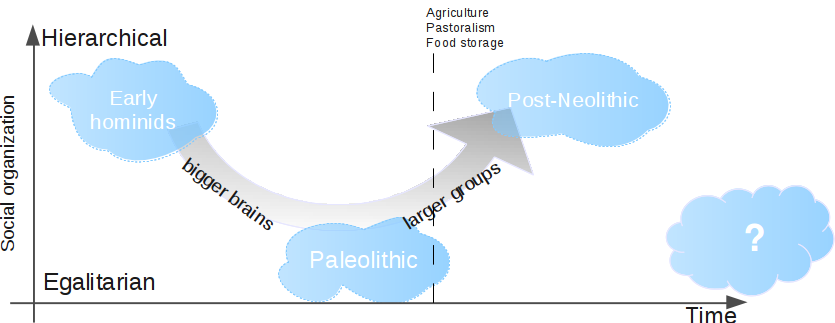
\includegraphics[width = \textwidth]{figuras/ushaped.png}
 	\caption{\label{fig:ushaped} Ilustração da história da organização social dos humanos e primatas pré-humanos.}
\end{figure}

\subsection{}

\subsection{Evolução do cérebro primata e a Teoria Maquiavélica}

Diversos trabalhos\cite{Dunbar2008,Dunbar2009, Dunbar2010,Aiello1993,Joffe1997} relacionam o tamanho relativo de regiões do cérebro de diversas espécies de primatas a medidas relacionadas com a capacidade social da espécie, como tamanho dos grupos em que vivem, o tamanho de coalizões, número médio de indivíduos que interagem diretamente, etc. O que é típicamente encontrado é ilustrado na figura \ref{fig:dunbarlaw}. Nessa figura mostra-se um gráfico do tamanho médio do grupo em função da razão média entre o volume do neo-córtex - região do cérebro dedicada ao planejamento, raciocínio, linguagem, entre outras funções cognitivas de ordem superior - e o volume total do cérebro para diversas espécies de primatas. O gráfico sugere uma relação do tipo lei de potência entre as duas grandezas, similar a encontradas em diversas outras comparações desse tipo. Em essência, essa relação sugere que a capacidade cognitiva dos primatas está intimamente relacionada a sua necessidade de dar conta de interações sociais cada 
vez mais complexas e sugere um cenário em que o rápido crescimento na importância relativa do neo-córtex é uma resposta a uma pressão seletiva associada a essa necessidade de interação social.  

\begin{figure}
	\centering
	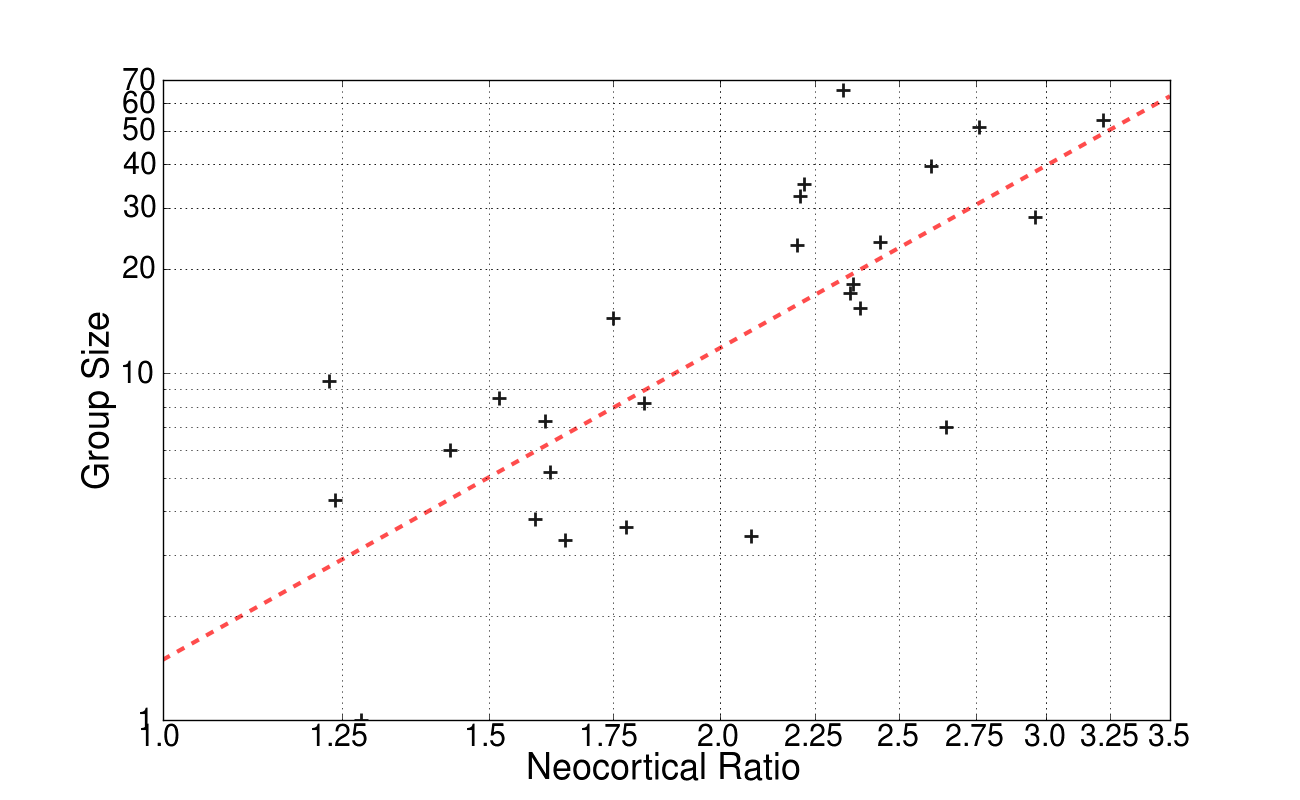
\includegraphics[width = \textwidth]{figuras/dunbar.png}
 	\caption{\label{fig:dunbarlaw} Gráfico em escala di-logaritimica do tamanho médio do grupo em função da razão média entre o volume do neo-córtex e o volume total do cérebro para diversas espécies de primatas. Dados disponíveis em \citep{Dunbar2009}.}
\end{figure}

\subsection{Dados etnoráficos (?)}
\section{Um modelo mecanico-estatístico baseado em agentes}
\subsection{Descrição dos agentes}

\newthought{O objetivo dessa seção é} descrever um modelo estatístico para a formação de estrutura social que seja tratável por técnicas comuns à mecânica estatística e teoria de informação e compatível com as informações experimentais descritas acima. O primeiro passo na descrição do modelo consiste na elaboração de uma dinâmica de comportamento para um conjunto de agentes hipotéticos, que será a dinâmica temporal microscópica que dará origem a um modelo mecânico-estatístico. 

\newthought{Considere um grupo de $n$ agentes} dotados de certa capacidade cognitiva limitada e engajados em atividades sociais. Cada agente carrega um registro mental da informação que possui a respeito das relações sociais entre os membros do seu grupo. Essa informação está relacionada a como cada par de outros agentes do grupo se relaciona socialmente. Essa informação deve responder perguntas como: 
\begin{itemize}
 \item qual a possibilidade de esse par de individuos serem adversários em uma disputa ou aliados em uma coalizão?
 \item com que frequencia cooperam em uma atividade conjunta?
 \item como compartilham seus recursos um com o outro?
 \item etc...
\end{itemize}  
Cada agente adquire essa informação através de mecanismos diversos: através da história social do grupo, baseado no comportamento pregresso dos agentes; através de mecanismos de aprendizado social como fofoca (\textit{gossip}) em que a comunicação com outros agentes permite que o agente aprenda sobre experiências de outros; etc. Uma vez adquirida, essa informação é critica para subsidiar decisões sociais a serem tomadas pelo agente: com que grupo de agentes fazer uma coalizão, quando esperar cooperação de um certo indivíduo, etc. Erros em decisões podem custar recursos e posição social, e influenciar negativamente a capacidade reprodutiva do agente. Portanto, espera-se que uma espécie de agentes que tenha surgido por evolução via seleção natural tenha mecanismos congnitivos adequados para tentar minimizar esses erros em algum sentido. 

\newthought{A aquisição desse tipo de informação social} é uma atividade cognitivamente custosa. A capacidade limitada de processar essas informações implica que para mantê-las atualizadas, o indivíduo precisa desviar recursos 
que poderiam ser aplicados em outras atividades - coleta de alimentos, construção de abrigos, etc. Há evidências \cite[-5em]{deWaal2007,deWaal1990}\sourcesneeded de que o rastreamento de relações sociais demanda um considerável tempo dos individuos adultos em tribos de chimpanzés e humanos. Conforme se aumenta o tamanho do grupo, esse custo cresce com o número de ligações sociais possíveis e, portanto, quadraticamente com o número de indivíduos. Isso pode pode tornar a estratégia de adquirir e manter informações sobre todas as ligações sociais possíveis no grupo pouco adaptativa. Pode ser preferível ao agente nesse caso obter apenas informação sobre certas ligações sociais importantes e fiar-se em heurísticas para inferir as outras relações sociais (regras como ``amigo do amigo é amigo'', etc\ldots{}).

\newthought{Dessa forma, o modelo consistirá} dos seguintes elementos: muitos \emph{agentes} que interagem entre si, cada um carregando uma \emph{representação mental da estrutura social} do grupo a que pertence e individualmente tentando \emph{minimizar custos} associados a carregar esass informações sociais. Abaixo discutiremos uma representação matemática de cada um desses elementos. 

\subsection{Variáveis dinâmicas - grafos sociais}

\newthought{A realização matemática} da representação mental da estrutura social que cada agente carrega será feita através de grafos. A cada agente está associado um grafo cujos nós representam todos os indivíduos do grupo e arestas representam as relações sociais sobre as quais o agente possui informação. A informação será considerada binária: o agente pode ter certeza sobre a relação social entre dois individuos, havendo portanto uma aresta ligada entre os nós correspondentes de seu grafo, ou não tem nenhuma informação direta sobre ela, caso em que não haverá uma aresta enter os nós correspondentes. As arestas do grafo portanto podem estar apenas ligadas ou desligadas, sem estados intermediários. As arestas do grafo são entidades dinâmicas, que podem ser criadas quando o agente adquire informação sobre uma relação social anteriormente desconhecida, ou destruídas quando o agente, por alguma razão, desiste de continuar mantendo aquela informação. Dados os custos, que serão discutidos abaixo, o agente deverá decidir quais informações valem a pena ser guardadas ou não. Um agente que possui informação completa sobre todas as relações sociais do grupo tem um grafo totalmente conectado, como o representado na figura \ref{fig:graph1}. 
\begin{marginfigure}[-45em]
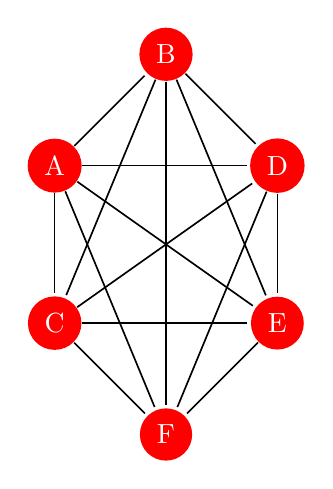
\begin{tikzpicture}[every node/.style={circle,white,fill=red}, shorten >= 1pt, auto, node distance =2cm, semithick]
   \node     (A)                    {A};
   \node     (B) [above right of=A] {B};
   \node     (C) [below of=A]       {C};
   \node     (D) [below right of=B] {D};
   \node     (E) [below of=D]       {E};
   \node     (F) [below right of=C] {F};
   \draw (A) -- (B);
   \draw (A) -- (C);
   \draw (A) -- (D);
   \draw (A) -- (E);
   \draw (A) -- (F);
   \draw (B) -- (C);
   \draw (B) -- (D);
   \draw (B) -- (E);
   \draw (B) -- (F);
   \draw (C) -- (D);
   \draw (C) -- (E);
   \draw (C) -- (F);
   \draw (D) -- (E);
   \draw (D) -- (F);
   \draw (E) -- (F);
 \end{tikzpicture}
 \caption[Grafo totalmente conectado]{Exemplo de grafo social - um grafo completamente conectado. Um agente com essa estratégia despende recursos para conhecer todas as relações sociais do grupo. Um grafo como esse possui $\frac{1}{2} n(n-1)$ arestas, onde $n$ é o número de agentes.}
 \label{fig:graph1}
 \end{marginfigure}
 
 \newthought{Quando uma aresta é faltante} no grafo carregado por um agente, a informação social correspondente à essa aresta é incompleta - o agente não tem informação direta sobre essa, e o agente deve recorrer a heuristicas para determinar quaisquer informações necessárias. Para tal, vamos considerar que o grafo deve ser conexo - deve ser possível, para todos os pares de nós, encontrar um \emph{caminho} de arestas ligadas conectando os dois nós. Dessa forma, sempre é possível a um agente determinar alguma informação indireta enter dois nós desconexos, através de uma heuristica que utilize as outras arestas conhecidas. Um exemplo é o grafo da figura \ref{fig:graph2}, que representa um grafo do tipo estrela. 
  \begin{marginfigure}[-10em]
 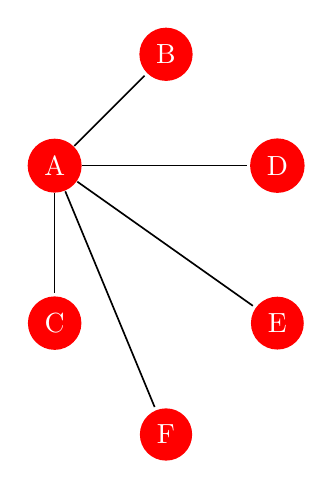
\begin{tikzpicture}[every node/.style={circle,white,fill=red}, shorten >= 1pt, auto, node distance =2cm, semithick]
   \node  (A)                    {A};
   \node  (B) [above right of=A] {B};
   \node  (C) [below of=A]       {C};
   \node  (D) [below right of=B] {D};
   \node  (E) [below of=D]       {E};
   \node  (F) [below right of=C] {F};
   \draw (A) -- (B);
   \draw (A) -- (C);
   \draw (A) -- (D);
   \draw (A) -- (E);
   \draw (A) -- (F);
\end{tikzpicture}
\caption[Grafo estrela]{Exemplo de grafo social - um grafo estrela. Um agente com essa estratégia despende recursos para conhecer apenas as relações envolvendo um certo indivíduo central (o nó A na figura). As outras relações são determinadas através de regras heurísticas. Esse grafo possui $n-1$ arestas.}
\label{fig:graph2}
\end{marginfigure}
Nesse grafo, não é possível conhecer diretamente todas as relações sociais pois apenas $n-1$ das $\frac{1}{2}n(n-1)$ arestas possíveis está presente. Mas todas as relações sociais podem ser indiretamente determinadas por heurísticas sobre caminhos de comprimento 2 (``amigo do amigo é amigo'', etc...). Os grafos mais esparsos possíveis que ainda são conexos possuem $n-1$ arestas, no mínimo.

\subsection{Custos}

\newthought{Existem custos associados} à manutenção de um certo grafo de informações sociais. Há principalmente dois tipos de custos:  
\begin{enumerate}

\item \newthought{O custo cognitivo} de adquirir e manter informação dos diferentes pares de individuos. Como discutido anteriormente, se o agente tem recursos cognitivos limitados, manter essas informações é custoso. Se assumirmos que o investimento de recursos para obter informações sobre cada aresta do grafo é constante, o custo cognitivo total por agente deverá ser proporcional ao número de arestas do grafo:
\begin{equation}
   H_{\text{cognitivo}} \propto n_{e}
\end{equation}
onde $n_{e}$ é o número de arestas (\emph{edges}).

\item \newthought{O custo social} de falhar em determinar corretamente a relação entre dois indivíduos. As heuristicas utilizadas pelo agente quando ele não possui informação direta sobre uma certa relação social podem falhar e, nesse caso, o agente pode comete um erro e tomar decisões baseadas nesse erro. Nesse caso existem custos - o agente pode avaliar incorretamente em que lado de uma disputa um individuo vai se posicionar, falhar em reconhecer uma coalizão em formação, etc, e ter prejuízos reais com uma situação social inesperada. As heuristicas que se valem de arestas conhecidas para inferir as relações desconhecidas devem tão menos confiáveis quanto maior o caminho mais curto no grafo entre os dois nós em questão. Quanto mais longos os trajetos a serem percorridos, maior é a probabilidade de erro. Portanto, o custo social esperado deve ser proporcional à distância geodésica média entre os nós do grafo:
\begin{equation}
 H_{\text{social}} \propto \frac{2}{n(n-1)} \sum_{i<j}{L_{ij}}
\end{equation}
onde $L_{ij}$ é a distância geodésica entre os nós $i$ e $j$, e a soma é realizada sobre todos pares de agentes. 

\end{enumerate}
O custo total para cada agente será dado, portanto, por:
\begin{equation}
   \label{eq:hamiltoniano}
   H = \frac{n_{e}}{\alpha}  + \bar{L}
\end{equation}
Onde $\bar{L}$ é a distancia geodésica média do grafo, $\alpha$ é uma constante associada à capacidade cognitiva do agente (quanto maior $\alpha$, menos importante é o custo cognitivo). Note que tipicamente $n_{e}$ escala como uma fração do número total de arestas possíveis $n(n-1)/2$ e que $\bar{L}$ escala tipicamente com $\log(n)$ para grafos aleatórios. É, portanto, interessante, reescrever (\ref{eq:hamiltoniano}), a menos de uma constante multiplicativa, como:
\begin{equation}
   \label{eq:hamiltoniano2}
   H = \phi_{e}  + a \bar{L}
\end{equation}
onde $\phi_{e} = \frac{n_{e}}{n(n-1)/2}$ é a fração de arestas ocupadas e $a = \frac{2\alpha}{n(n-1)}$ é uma constante de acoplamento: a capacidade cognitiva média dedicada a cada aresta. 

\subsection{Dinâmica para agentes isolados - máxima entropia}
\newthought{Para que um modelo possa ser estabelecido}, não basta a expressão para o custo, mas uma descrição de que ações o agente deverá tomar com base em sua aferição do custo. A estratégia do agente é definida por uma certa escolha de arestas a investir. Em uma primeira abordagem, atribuimos ao agente a tendência a usar a estratégia que minimiza o custo total. Então deveriamos procurar pelo grafo definido por:
\begin{equation}
\label{eq:minimize}
  G_{\star}(\alpha) = \arg\min_{G} H(G,\alpha)
\end{equation}
Se $\alpha \gg 1$, então as limitações cognitivas são menos e menos importantes. O grafo que minimiza o custo é o grafo que minimiza a distância geodésica média - um grafo totalmente conectado como o da figura \ref{fig:graph1}. Se \(\alpha \ll 1\), então as limitações cognitivas se tornam mais e mais importantes, e o grafo ótimo é aquele que minimiza o número de arestas, enquanto ainda mantendo uma distância média finita - um grafo em forma de estrela \footnote{Estritamente para \(\alpha = 0\) o grafo ótimo é o grafo sem aresta alguma. Não há prescrição canônica para a distância geodésica média de um grafo sem arestas. Adotaremos aqui a convenção de que se não é possível desenhar um caminho entre dois nós (em outras palavras: dois nós que pertencem a diferentes componentes do grafo), então a distância entre eles é infinita. Isso restringe nossa análise apenas a grafos conexos. Mesmo entre os grafos conexos, a estrela não é o único mínimo do custo acima para \(\alpha\) estritamente zero - o grafo caminho 
também é possível. Entretanto, para o grafo caminho, \(\bar{L}\) é proporcional a \(N\), e portanto, para $\alpha \to +0$ o único mínimo existente quando $\alpha > 0$ tem grafo estrela como limite. } como o da figura \ref{fig:graph2}. Para valores intermediários de \(\alpha\), o grafo ótimo possui configurações intermediárias entre esses dois extremos. 

\newthought{Podemos  relaxar o vínculo de estrita minimização} e propor o seguinte modelo: o agente decide sua estratégia através de uma dinamica interna que ocorre em seu cérebro, ditada por regras que levam em conta o custo total. Podemos então associar probabilidades às estratégias de acordo com nossa expectativa de que grafos devem surgir dessa dinâmica. Se não conhecemos detalhes da dinâmica, mas temos informação de que o valor esperado do custo total é uma variável importante, o procedimento bayesiano adequado é associar ao grafo uma distribuição de máxima entropia, restringida pelo valor do custo total. A distribuição resultante é a distribuição de Gibbs:
\begin{equation}
   \label{eq:gibbs}
   p(G) = \frac{q(G)}{Z} e^{-\beta H(G)}
\end{equation}
onde $\beta$, uma espécie de inverso de temperatura, regula a importância relativa dos efeitos que o custo \(H(G)\) e outros efeitos negligenciados pelo modelo, e \(q(G)\) é a atribuição de probabilidades a priori. Assumiremos probabilidades uniformes a priori, com a restrição de que o grafo seja conexo (veja nota \footnotemark[\value{footnote}]).A atribuição de probabilidades da equação (\ref{eq:gibbs}) torna o problema de determinar as propriedades macroscópicas desse sistema em um problema de mecânica estatística, cuja variável dinâmica é a matriz de adjacências do grafo G:
\begin{equation}
  M_{ij} = \begin{cases}
      1  & \text{se $i$ e $j$ estão ligados por uma aresta} \\
      0  & \text{outro caso}
           \end{cases}
\end{equation}
\subsection{Interpretação do parâmetro $\beta$}
\subsection{Resultados numéricos para agentes isolados}
\newthought{Simulações de Monte Carlo} desse modelo foram feitas usando o algoritmo de Metrópolis. Partindo de um grafo inicial aleatório (sorteado do ensemble de Erdos-Renyi, com fração de arestas $\frac{1}{2}$), a cada passo do algoritmo é proposta uma mudança em uma aresta do grafo - adicionando uma aresta faltante ou removendo uma aresta existente. Caso a mudança não quebre a conectividade do grafo, ela será aceita com probabilidade dada pelo fator de Gibbs: 
\begin{equation}
\label{eq:gibbsfactor}
e^{-\beta \left(H(G') - H(G)\right)}.
\end{equation}

\begin{figure}
  \includegraphics[width = 1.1\textwidth]{figuras/cutstar.png}
  \caption[Corte do diagrama de fases apresentando a média térmica obtida via  Monte Carlo.]{\label{fig:cutstar} Corte do diagrama de fases apresentando a média térmica obtida via  Monte Carlo dos parâmetros de ordem normalizados $\dmax$ e $\davg$ em função de $\alpha$, com temperatura e número de agentes fixo, bem como seus desvios padrão. Sobreposto ao gráfico se observam exemplos de arquiteturas do grafo sorteadas da distribuição de equilibrio na região correspondente do diagrama. }
\end{figure}
\begin{fullwidth}
\begin{figure}
	\includegraphics[width = 2.1\textwidth, angle=90]{figuras/phasediagram.png}
 	\caption{\label{fig:phasediagram} Diagrama de fases apresentando a razão $\frac{\davg}{\dmax}$ em função de $\alpha$ e temperatura, para um número fixo de agentes.}
\end{figure}
\end{fullwidth}
\newthought{Na figura} \ref{fig:cutstar} temos um corte do diagrama de fase desse modelo com temperatura e número de agentes constante, variando o parâmetro $\alpha$. Seja $d_i$ o grau do $i$-ésimo nó do grafo de um agente escolhido ao acaso. No painel superior destacamos dois parâmetros de ordem: $\dmax = \frac{1}{N-1}\max\left(d_1, d_2,\ldots, d_N\right)$, em azul, é proporcional ao grau do nó mais bem conectado do grafo, e $\davg = \frac{1}{N(N-1)}\sum_{i=1}^N d_i$, em vermelho, é proporcional ao grau médio de todos os nós do grafo. Uma vez que o maior possível grau para um nó é $N-1$, esses parâmetros foram normalizados para que o valor máximo seja 1. As linhas sólidas correspondem à média térmica obtida através da simulação de Monte Carlo do modelo, enquanto o sombreado ao redor da linha representa o desvio padrão obtido da mesma forma. No painel inferior apresentamos novamente o desvio padrão para melhor visualização. Sobrepostas aos gráficos estão figuras representativas de grafos sorteados da 
distribuição de equilíbrio em pontos correspondentes do diagrama de fases. Como observado anteriormente, para $a = \frac{2\alpha}{N(N-1)}$ pequeno - baixa capacidade cognitiva, ou grupos grandes - há uma fase em que o grafo se organiza como uma estrela. Para $a$ grande - alta capacidade cognitiva ou grupos pequenos - o grafo tem conectividade densa, tendendo a um grafo totalmente conectado conforme o parâmetro aumenta. 

\begin{figure}
	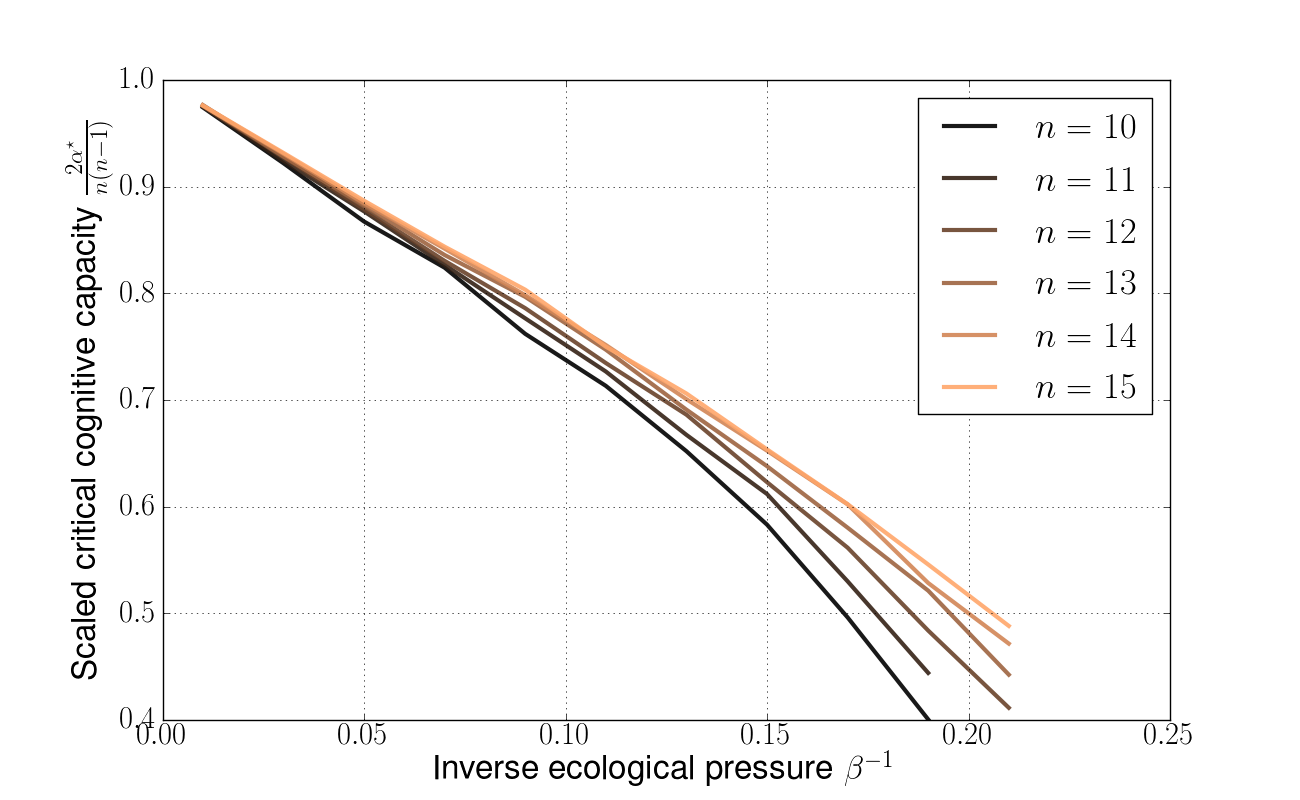
\includegraphics[width = 1.15\textwidth]{figuras/critical.png}
 	\caption{\label{fig:critical} Valor crítico do parâmetro $a$ em função da temperatura para diferentes tamanhos do sistema.}
\end{figure}	

\newthought{Uma caracteristica é interessante} na região intemediária, entretanto: o grafo continua com um nó fortemente central e baixa conectividade na periferia para valores de $a$ relativamente grandes, até que uma repentina mudança de comportamento, acompanhada de um pico nas variâncias dos parâmetros de ordem, indicando uma aparente transição de fase. Nessa segunda fase, a conectividade do nó mais central já não é mais máxima, e a conectividade dos nós periféricos é comparável à do nó central. Conforme $a$ cresce, o grafo tende a se tornar totalmente conectado, com valores de $\dmax$ e $\davg$ compativeis com os de um grafo no ensemble de Erdos-Renyi (um grafo aleatório, com número médio de arestas fixo).


\newthought{Na figura}\ref{fig:phasediagram} temos um diagrama de fases completo variando $\alpha$ e a temperatura para um número fixo de agentes. A variável descrita no mapa de cores é a razão $\frac{\davg}{\dmax}$. Esse diagrama mostra uma linha de transição de fases entre a região azul escura - a região em que a organização do grafo é fortemente centralizada, com nós periféricos pouco conectados, e uma região em que a razão $\frac{\davg}{\dmax}$ é menos extrema. Acima de uma temperatura crítica essa fase não é mais observada. A região vermelho escura corresponde à fase totalmente conectada, ou situações bem próximas disso. Nessa região não há grandes saltos nos parâmetros de ordem, que mudam continuamente com a temperatura e $a$. A linha de transição de fase pode ser observada para diferentes valores da temperatura na figura \ref{fig:critical}. Note que para $\beta^{-1} \to 0$, temos $\alpha^{\star} = 1$.


\subsection{Dinâmica para muitos agentes } 

\newthought{As figuras acima} tratam de propriedades independentes da interação entre os agentes. Essa interação, como dito anteriormente, será introduzidas na forma de aprendizado social (``fofoca'' ou \textit{gossip}). Durante a simulação de Monte Carlo, com uma certa probabilidade $g$, dois agentes são sorteados e trocam informação uma aresta com probabilidade proporcional ao fator de Gibbs \eqref{eq:gibbsfactor}. Esse procedimento visa imitar o aprendizado social observado em humanos \cite[-2em]{Dunbar2010book}. Essa escolha de interação não altera os diagramas já mostrados, mas introduz correlação entre os grafos de diferentes agentes. 
\begin{figure}
	\centering
	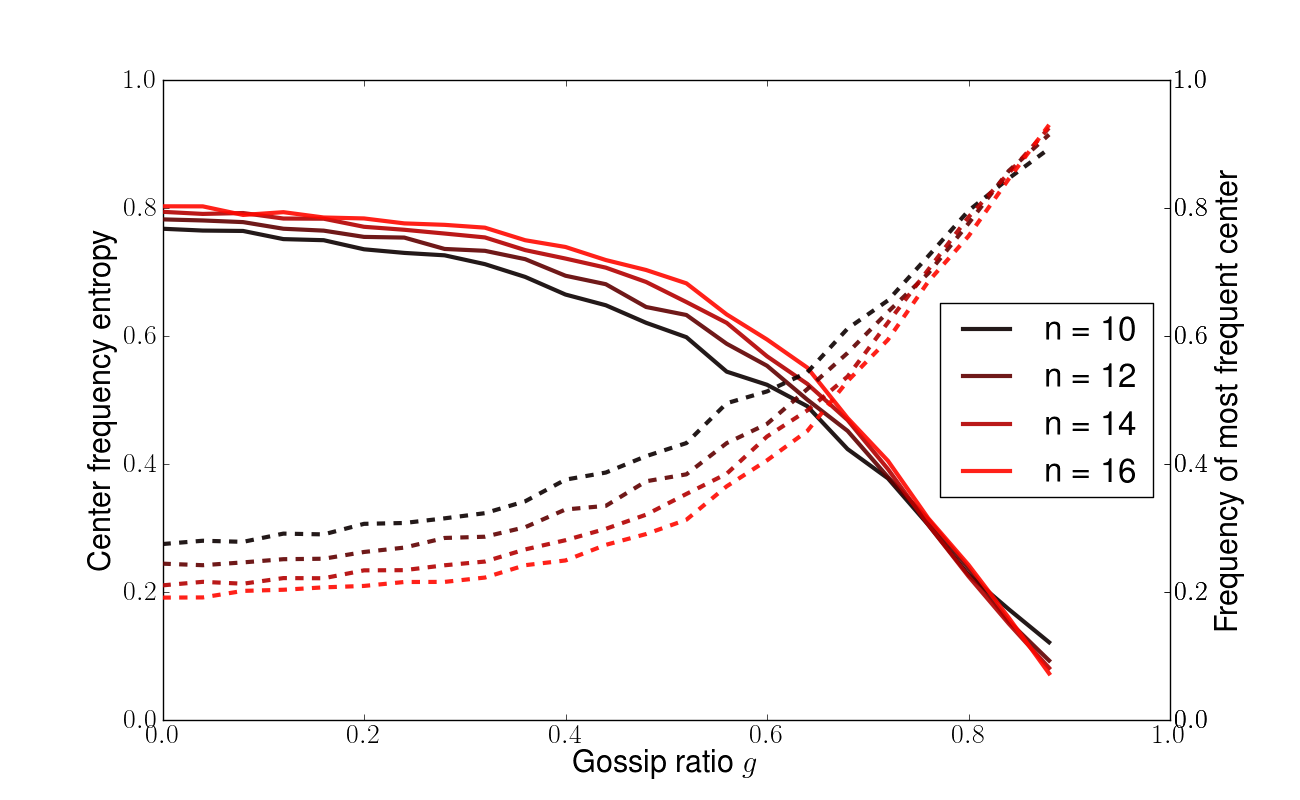
\includegraphics[width = 1\textwidth]{figuras/gossip.png}
 	\caption[Parâmetros de ordem associados à correlação entre grafos de diferentes agentes]{\label{fig:gossip} Parâmetros de ordem associados à correlação entre grafos de diferentes agentes, calculados na fase em que os grafos apresentam estrutura de estrela. As curvas tracejadas correspondem à frequência do nó central mais frequente. As linhas tracejadas correspondem à entropia da distribuição de centros.}
\end{figure}
Na figura \ref{fig:gossip} são exibidas duas grandezas que quantificam a correlação entre os grafos na fase estrela. Vamos denotar por $c_i$ o label que identifica o nó central do grafo do $i$-ésimo agente. Para um certo número $N$ de agentes temos então o conjunto $\{c_1, c_2, \ldots, c_N\}$. Seja a variável aleatória $c$ definida como um valor sorteado ao acaso desse conjunto. A primeira grandeza do grafo, correspondente às linhas tracejadas, é dada por $\max_{c} \Prob(c)$, ou seja, a frequencia do agente que mais frequentemente é o centro de algum grafo naquele passo do algoritmo. Isso corresponde de forma grosseira a que fração dos agentes tem grafos estrela com o mesmo nó ocupando o centro da estrela. A segunda variável é, a menos de uma constante multiplicativa, simplesmente a entropia da distribuição de $c$: $S(c) = -\sum_{c} \Prob(c) \log\Prob(c)$. Ambas as grandezas são calculadas para grafos em forma de estrela, em função da probabilidade de encontro entre dois agentes dada por $g$, para valores 
fixos de temperatura, variando-se o número de agentes. O resultado mostra que, para baixos valores de $g$, a probabilidade de que um certo nó seja o centro de um agente tomado ao acaso é aproximadamente uniforme, e nenhum dos nós domina como centro de uma fração substancial de grafos. Para valores maiores de $g$, os grafos estrela tendem a se correlacionar e o mesmo nó pode ser central em uma grande fração de agentes. 

\newthought{É possível}, dessa forma, distinguir três situações, ou ``fases'' desse modelo:
\begin{enumerate}
 \item Para $a$ grande, ou seja, grupos de tamanho pequeno ou agentes com grande capacidade cognitiva, os agentes possuem modelos mentais do panorama social do seu grupo em que nenhum agente em particular ocupa uma posição central. Em outras palavras, a representação mental das redes sociais nesse grupo são todas simétricas e nenhum agente se destaca. 

 \item Para $a$ pequeno e $g$ pequeno, ou seja, grupos de tamanho grande ou agentes com capacidade cognitiva pequena, e pouca interação social, cada agente possui um modelo mental da paisagem social que privilegia um dos agentes como central na definição de todas as relações sociais do grupo. Suas decisões em jogos sociais são tomadas levando em conta a natureza das relações sociais de todos os agentes com esse agente central. Entretanto os nós centrais de cada agente são sorteados aleatóriamente e, de certa forma, apesar de haver uma quebra de simetria na representação mental que cada agente faz do grupo, a situação global ainda é simétrica. 

 \item Para $a$ pequeno e $g$ grande,  ou seja, grupos de tamanho grande ou agentes com capacidade cognitiva pequena, e interação social intensa, todos os agentes possuem o mesmo modelo mental: uma rede social centrada em torno de um agente específico, que se torna a medida de todas as relações sociais no grupo. Todo agente do grupo usa as conexões desse mesmo agente central como informação mais relevante na tomada de decisões em jogos sociais. Esse agente central está posicionado de forma privilegiada como central na solução de dilemas sociais, formação de coalizões e outras atividades sociais do grupo. 
\end{enumerate}
Postulando que o capital social derivado dessa posição central quebra a simetria do resultado desses jogos sociais de maneira vantajosa ao agente central, esse resultado é compatível com as observações empíricas descritas no inicio do texto. 
\ldots
\subsection{Resultados numéricos para muitos agentes}
\section{Sumarização e interpretação dos Resultados}
\section{Conclusão}
